\section{Auswertung}
\subsection{Kontrastmessung}
Zunächst muss für eine bessere Qualität der späteren Messung der Kontrast
ermittelt werden. Mit Hilfe von Formel \eqref{eqn:kontrast} wird dieser
berechnet. Die gemessenen Spannungen mit den zugehörigen Winkeln werden in
Tabelle \ref{tab:kontrast} dargestellt.

\begin{table}
[H]
  \centering
\begin{tabular}{cccc}

  \toprule
$\phi \ [\si{\degree}]$ & $U_\text{min} \ [\SI{}{\volt}]$ &
$U_\text{max} \ [\SI{}{\volt}]$ & $K$ \\
\midrule

195 & \SI{1.28}{} & \SI{2.70}{} & \SI{0.36}{} \\

180 & \SI{1.52}{} & \SI{1.82}{} & \SI{0.09}{} \\

165 & \SI{0.76}{} & \SI{2.01}{} & \SI{0.45}{} \\

150 & \SI{0.24}{} & \SI{1.70}{} & \SI{0.75}{} \\

135 & \SI{0.06}{} & \SI{1.30}{} & \SI{0.91}{} \\

120 & \SI{0.10}{} & \SI{0.95}{} & \SI{0.81}{} \\

105 & \SI{0.26}{} & \SI{0.82}{} & \SI{0.52}{} \\

90  & \SI{0.67}{} & \SI{0.81}{} & \SI{0.09}{} \\

75  & \SI{0.47}{} & \SI{1.57}{} & \SI{0.54}{} \\

60  & \SI{0.15}{} & \SI{2.66}{} & \SI{0.89}{} \\

45  & \SI{0.14}{} & \SI{3.41}{} & \SI{0.92}{} \\

30  & \SI{0.54}{} & \SI{3.13}{} & \SI{0.71}{} \\

15  & \SI{1.21}{} & \SI{2.75}{} & \SI{0.39}{} \\

0   & \SI{1.64}{} & \SI{1.90}{} & \SI{0.07}{} \\

-15 & \SI{0.70}{} & \SI{2.00}{} & \SI{0.48}{} \\

\bottomrule
\end{tabular}

\caption{Berechneter Kontrast in Abhängigkeit der Polarisationsrichtung}
\label{tab:kontrast}
\end{table}



Nach Auftragen der Messwerte kann auf einen Zusammenhang geschlossen werden,
der der Betragsfunktion des Sinus ähnelt. Die Ausgleichsfunktion lautet somit
\begin{equation}
  f(\phi) = a \cdot \lvert \sin(b \cdot \phi +c) \rvert +d
\end{equation}
Die Messwerte und die Ausgleichsfunktion sind in Abbildung \ref{fig:kontrast}
dargestellt.

Für die Parameter ergeben sich die folgenden Werte
\begin{align*}
  a &= \SI{0.88 \pm 0.05}{} \\
  b &= \SI{2.00 \pm 0.02}{\per\radian} \\
    &\hat{=}\, \SI{114.82 \pm 1.03}{\per\degree} \\
  c &= \SI{-0.06 \pm 0.04}{} \\
  d &= \SI{0.03 \pm 0.03}{} \\
\end{align*}

Der Parameter $a$ beschreibt die Amplitude, $b$ eine Frequenz, $c$ die
Phasenverschiebung und $d$ den Kontrastoffset.
Zur Berechnung des optimalen Polarisationswinkel wird das Maximum der
Ausgleichsfunktion ermittelt.
\begin{equation}
  \phi = \frac{1}{b} \left(\frac{\pi}{2} -c \right)
\end{equation}
Dadurch ergibt sich ein Winkel von
\begin{align*}
  \phi &= \SI{0.82}{\radian} \\
       &\hat{=} \, \SI{46.72}{\degree} \\
\end{align*}
Der Fehler berechnet sich mit Hilfe der Gaußschen Fehlerfortpflanzung
\begin{equation}
  \Delta \phi =\sqrt{\left(- \frac{1}{b^2} \left(\frac{\pi}{2} -c \right)  \right)^2
  \Delta b^2 + \left(- \frac{1}{b}\right)^2 \Delta c^2}
\end{equation}

\begin{figure}[H]
  \centering
  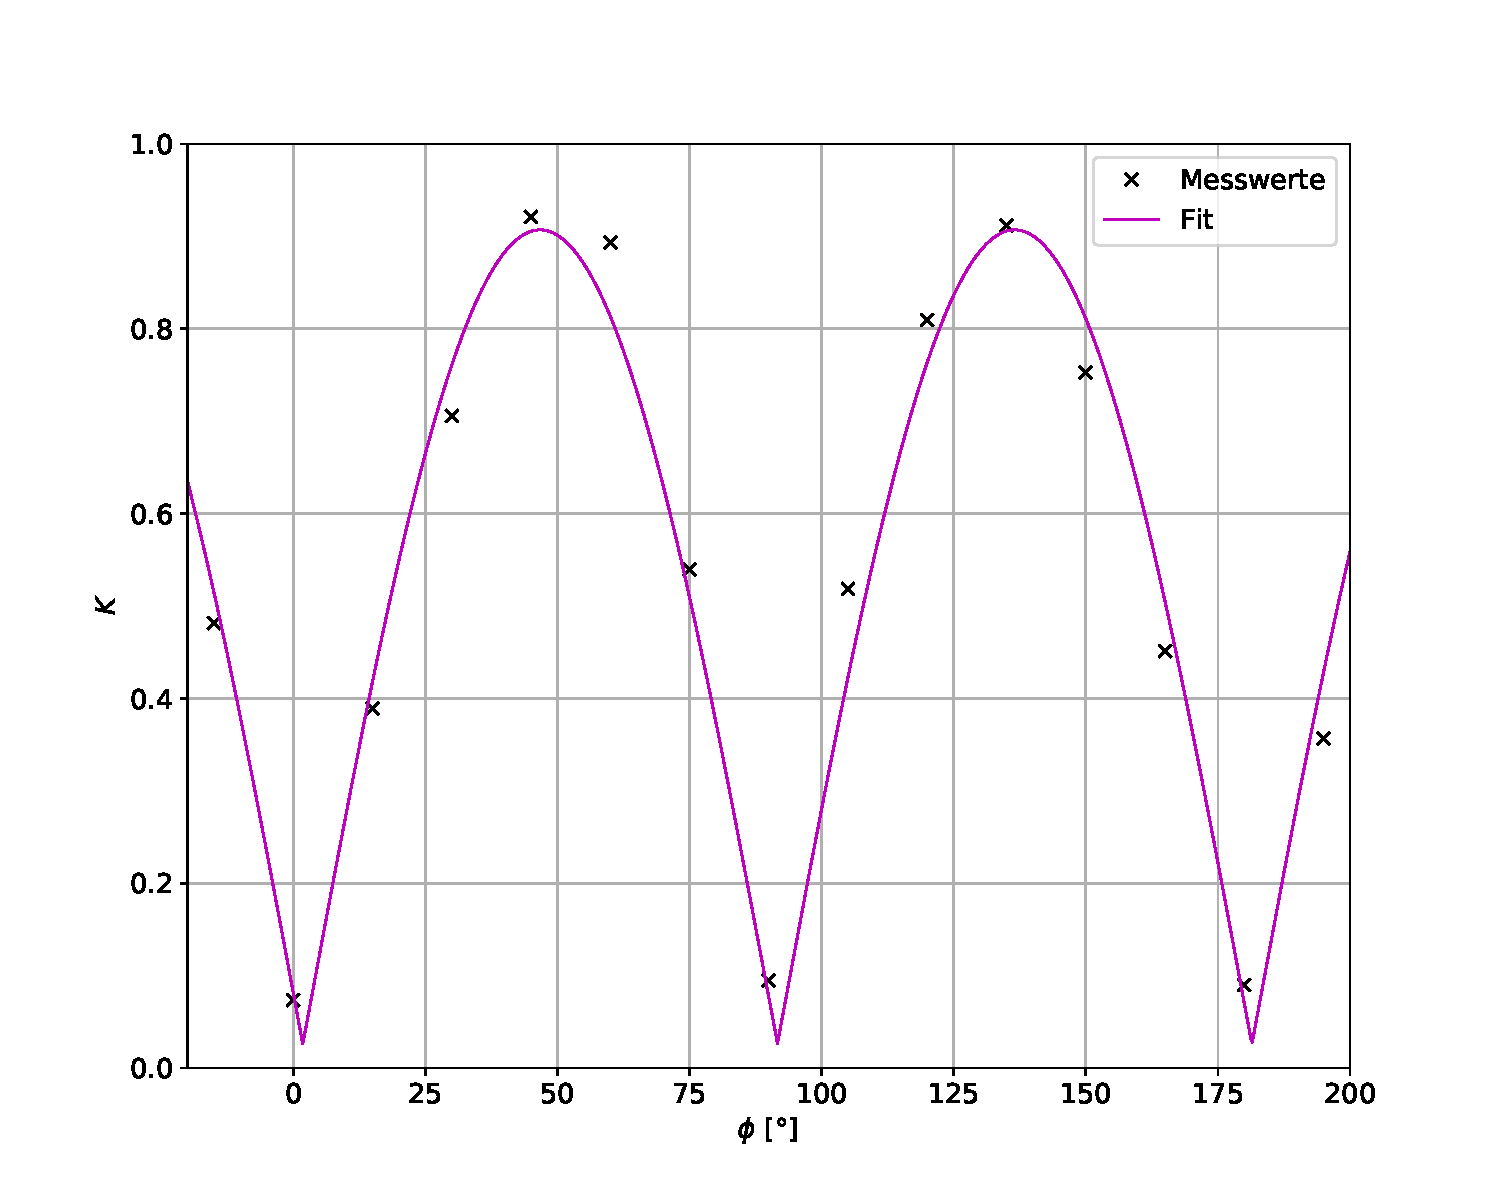
\includegraphics[width=\textwidth]{kontrast.pdf}
  \caption{Kontrast in Abhängigkeit der Polarisationsrichtung mit
  Ausgleichsrechnung}
  \label{fig:kontrast}
\end{figure}
\subsection{Berechnung des Brechungsindex von Glas}
Die gemessenen Maxima mit den zugehörigen Winkeländerungen sind in Tabelle
\ref{tab:glas} dargestellt. Der Brechungsindex berechnet sich mit Hilfe
der Formel \ref{eqn:glas}. Die zugehörigen Brechunsindizes sind neben den
Wertepaaren aufgelistet.

\begin{table}
  \centering
\begin{tabular}{SSSSSSSSS}
  \toprule
  \multicolumn{3}{c}{Messung 1} &\multicolumn{3}{c}{Messung 2}
  & \multicolumn{3}{c}{Messung3} \\
$\phi \, [\si{\radian}]$ & $M$ & $n$ & $\phi \, [\si{\radian}]$ & $M$ & $n$ &
 $\phi \, [\si{\radian}]$ & $M$ & $n$\\
2 & 6 & 1.451 & 2 & 6 & 1.451 & 2 & 5 & 1.35 \\

2 & 7 & 1.569 & 2 & 7 & 1.569 & 2 & 6 & 1.451 \\

2 & 8 & 1.708 & 2 & 7 & 1.569 & 2 & 8 & 1.708 \\

2 & 7 & 1.569 & 2 & 6 & 1.451 & 2 & 7 & 1.569 \\

2 & 6 & 1.451 & 2 & 7 & 1.569 & 2 & 6 & 1.451 \\

\bottomrule
\end{tabular}
\caption{Gemessene Anzahl der Maxima pro Winkeländerung}
\label{tab:glas}
\end{table}


Es ergibt sich ein Mittelwert mit der zugehörigen Standartabweichung von
\begin{align*}
  \bar{n} = \SI{1.526 \pm 0.097}{} \, .\\
\end{align*}

Die Herstellerangabe \cite{skript} für den Brechungsindex lautet

\begin{align*}
  n_H = \SI{1.5}{} \, .
\end{align*}

Das entspricht einer prozentualen Abweichung von $\SI{0.017}{\%}$.

\subsection{Berechnung des Brechungsindex von Luft}

Für die Messungen des Brechungsindex von Luft ergeben sich folgende Werte
\begin{align*}
  \text{Messung 1} &= \SI{42}{} \text{Counts} \\
  \text{Messung 2} &= \SI{42}{} \text{Counts} \\
  \text{Messung 3} &= \SI{42}{} \text{Counts} \, . \\
\end{align*}
Es muss beachtet werden, dass kein vollständiges Vakuum erreicht werden konnte
und das der Wert des erreichten Normaldrucks nicht dem üblichen Wert von
$p_a= \SI{1013}{\milli\bar}$ \cite{druck} entspricht. Die erreichten Druckwerte sind in
diesem Versuch die Folgenden.
\begin{align*}
  p_{\text{min}} &= \SI{1002}{\milli\bar} \\
  p_0            &= \SI{5}{\milli\bar} \\
\end{align*}

Zur Berechnung des Brechungsindes von Luft wird Formel \ref{eqn:brechluft}
verwendet. Die Länge der Messzelle $L$ und die Wellenlänge des Lasers
haben dabei die folgenden Werte.

\begin{align*}
  L &= \SI{100 \pm 0.1}{\milli\meter} \\
  \lambda &= \SI{632.990}{\nano\meter} \\
\end{align*}

Dadurch ergeben sich für die einzelnen Messung die folgenden Brechunsindizes.
\begin{align*}
  n_1 &= \SI{1.000133}{} \\
  n_2 &= \SI{1.000133}{} \\
  n_3 &= \SI{1.000133}{} \\
\end{align*}
Wird lediglich der Fehler der Messzelle berücksichtig, so ergibt sich mittels
Gaußscher Fehlerfortpflanzung ein Wert von
\begin{align*}
  n = \SI{1.0001}{} \pm (\SI{1.3}{} \cdot 10^{-7}) \, .\\
\end{align*}
Dies ist jedoch ein Fehler der nicht der Messung entspricht. Beim Vakuumieren
der Gaszelle ist auf dem Oszilloskop eine Sinusschwingung zu erkennen. Diese
Schwingungen entsprechen dabei den durchlaufenden Interferenzmaxima. Nachdem
die Zelle vollständig vakuumiert wird, ist trotzdem noch eine getreckte
Sinusschwingung zu erkennen. Das Messgerät misst einen Count, wenn die
Sinusschwingung die Nulllinie übertritt und fast ihr Maximum erreicht. Das
Bedeutet, dass es eine Auswirkung auf die Anzahl der Counts hat, wo die
Messung begonnen wird. Das ist eine Fehlerquelle die mit einberechnet werden
muss. Da die Counts nur diskrete Werte annehmen können, wird dem Messwert
der Counts auch ein diskreter Fehler zugeordnet

\begin{align*}
  M &= 41 \pm 1 \, .\\
\end{align*}

Der Fehler berechnet sich dann mit Hilfe der Gaußschen Fehlerfortpflanzung

\begin{align*}
  \Delta{n} = \sqrt{\left( -\frac{M L}{2L} \right)^2 \cdot \Delta{L}^2
  + \left(\frac{\lambda}{2 L} \right)^2 \cdot \Delta{M}^2} \, .
\end{align*}
Dadurch ergibt sich für den Brechungsindex von Luft ein Wert von

\begin{align*}
n &= \SI{1.0001329 \pm 0.0000032}{} \, .
\end{align*}

Der Theoriewert für den Brechungsindex von Luft lautet
\begin{align*}
  n = \SI{1.000272}{} \, .
\end{align*}
Das entspricht einer Abweichung von $\SI{0.014}{\%}$.
